\documentclass{ximera}
\usepackage{OERLinearAlgebra}


\usepackage{mathtools}
\usepackage{tikz-3dplot}
\newcommand\norm[1]{\left\lVert#1\right\rVert}

\author{Anna Davis \and Rosemarie Emanuele} \title{Standard Unit Vectors in $\RR^n$} \license{CC-BY 4.0}

\begin{document}

\begin{abstract}
 We introduce standard unit vectors in $\RR^2$, $\RR^3$ and $\RR^n$, and express a given vector as a linear combination of standard unit vectors. 
\end{abstract}
\maketitle



\section*{Standard Unit Vectors in $\RR^2$ and $\RR^3$} 
A {\it unit vector} is a vector of length 1.  A unit vector in the positive direction of a coordinate axis is called a {\it standard unit vector}.  There are two standard unit vectors in $\RR^2$.  The vector $\vec{i}=\begin{bmatrix}
1\\
0
\end{bmatrix}$ is located along the $x$-axis, and the vector $\vec{j}=\begin{bmatrix}
0\\
1
\end{bmatrix}$ is located along the $y$-axis.  

\begin{image}[1.5in]
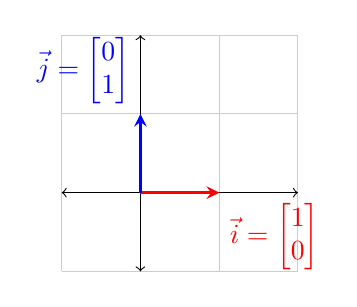
\begin{tikzpicture}[scale=1]
\draw[thin,gray!40] (-1,-1) grid (2,2);
  \draw[<->] (-1,0)--(2,0);
  \draw[<->] (0,-1)--(0,2);
  \draw[line width=1pt,-stealth, red](0,0)--(1,0) node[below right]{$\vec{i}=\begin{bmatrix}1\\0\end{bmatrix}$};
  
  \draw[line width=1pt,-stealth, blue](0,0)--(0,1) node[above left]{$\vec{j}=\begin{bmatrix}0\\1\end{bmatrix}$};
 \end{tikzpicture}
\end{image}

Vector names $\vec{i}$ and $\vec{j}$ are reserved for standard unit vectors in the direction of $x$ and $y$ axes, respectively.  We chose to express $\vec{i}$ and $\vec{j}$ as column vectors, instead of row vectors, because the context in which we will encounter them in the future will require them to be column vectors.  You may see them presented as row vectors in a different course.


There are three standard unit vectors in $\RR^3$: $$\vec{i}=\begin{bmatrix}
1\\
0\\
0
\end{bmatrix},\quad \vec{j}=\begin{bmatrix}
0\\
1\\
0
\end{bmatrix},\quad\vec{k}=\begin{bmatrix}
0\\
0\\
1
\end{bmatrix}$$

\begin{image}[3in]
\tdplotsetmaincoords{70}{130}
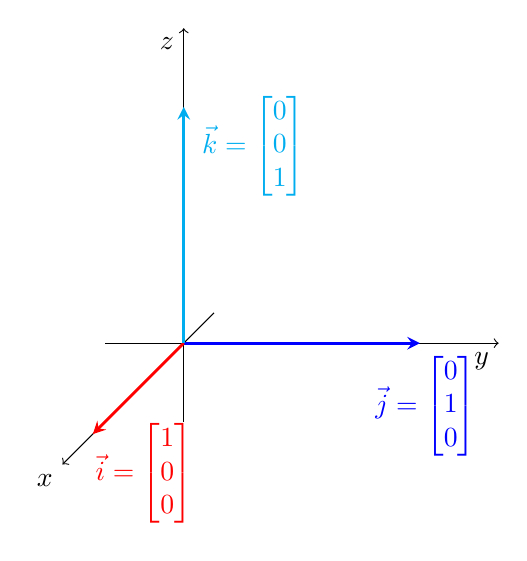
\begin{tikzpicture}
	\draw[->](-1,0,0)--(4,0,0) node[below left]{$y$};
    \draw[->](0,-1,0)--(0,4,0) node[below left]{$z$};
    \draw[->](0,0,-1)--(0,0,4) node[below left]{$x$};
        
    \draw[->, line width=1pt,blue, -stealth](0,0,0)--(3,0,0)node[below=0.8cm, right=-0.7cm]{$\vec{j}=\begin{bmatrix}0\\1\\0\end{bmatrix}$};
    
    \draw[->, line width=1pt,red, -stealth](0,0,0)--(0,0,3)node[below=0.5cm, right=-0.1cm]{$\vec{i}=\begin{bmatrix}1\\0\\0\end{bmatrix}$};
    
    \draw[->, line width=1pt,cyan, -stealth](0,0,0)--(0,3,0)node[below=0.5cm, right=0.1cm]{$\vec{k}=\begin{bmatrix}0\\0\\1\end{bmatrix}$};
   
    \end{tikzpicture}
\end{image}

\section*{A Vector as a Linear Combination of Standard Unit Vectors} 
Every vector in $\RR^2$ and $\RR^3$ can be written as a sum of scalar multiples of $\vec{i}$, $\vec{j}$ and $\vec{k}$.  For example, if $\vec{v}=\begin{bmatrix}
3\\
-2\\
7
\end{bmatrix}$, then
$$\vec{v}=\begin{bmatrix}
3\\
-2\\
7
\end{bmatrix}=\begin{bmatrix}
3\\
0\\
0
\end{bmatrix}+\begin{bmatrix}
0\\
-2\\
0
\end{bmatrix}+\begin{bmatrix}
0\\
0\\
7
\end{bmatrix}=3\begin{bmatrix}
1\\
0\\
0
\end{bmatrix}+(-2)\begin{bmatrix}
0\\
1\\
0
\end{bmatrix}+7\begin{bmatrix}
0\\
0\\
1
\end{bmatrix}=3\vec{i}-2\vec{j}+7\vec{k}$$

The expression $3\vec{i}-2\vec{j}+7\vec{k}$ is called a {\it linear combination} of $\vec{i}$, $\vec{j}$ and $\vec{k}$. 

%For an additional example, watch this Firefly Lectures Video:\\
%\href{https://www.youtube.com/watch?v=gY3hxwhqMhk}{https://www.youtube.com/watch?v=gY3hxwhqMhk}

\section*{Standard Unit Vectors in $\RR^n$}
When working with vectors in $\RR^n$ for $n>3$, we use different notation to denote the standard unit vectors.


  \begin{definition} 
  
  Let $\vec{e}_i$ denote a standard unit vector of $\RR^n$ which has 1 as the $i$th component and zeros elsewhere.  In other words, $$\vec{e}_i=\begin{bmatrix}
0\\
0\\
\vdots\\
1\\
\vdots\\
0
\end{bmatrix}$$ 
  where 1 is in the $i$th position.
\end{definition}


\section*{Practice Problems}
\begin{problem}
Express each of the following vectors as a linear combination of appropriate standard unit vectors.
  \begin{enumerate}
  \item 
  $$\vec{u}=\begin{bmatrix}
0\\
4\\
-3
\end{bmatrix}$$
Answer:
$$\vec{u}=\answer{0}\vec{i}+\answer{4}\vec{j}+\answer{-3}\vec{k}$$

\item 
$$\vec{v}=\begin{bmatrix}
-1\\
1
\end{bmatrix}$$
Answer:
$$\vec{u}=\answer{-1}\vec{i}+\answer{1}\vec{j}$$
\item 
$$\vec{w}=\begin{bmatrix}
5\\
-3\\
1\\
7
\end{bmatrix}$$
Answer:
$$\vec{u}=\answer{5}\vec{e}_1+\answer{-3}\vec{e}_2+\answer{1}\vec{e}_3+\answer{7}\vec{e}_4$$
  \end{enumerate}
\end{problem}

\begin{problem}
Express each given vector in component form.
  \begin{enumerate}
  \item 
  $\vec{u}=\vec{i}+3\vec{j}$ is a vector in $\RR^2$.
  
  Answer:
  $$\vec{u}=\begin{bmatrix}\answer{1}\\\answer{3}\end{bmatrix}$$
  \item
  $\vec{v}=-\vec{j}+5\vec{k}$ is a vector in $\RR^3$.
  
  Answer:
  $$\vec{v}=\begin{bmatrix}\answer{0}\\\answer{-1}\\\answer{5}\end{bmatrix}$$
  \item
  $\vec{w}=\vec{e}_1-2\vec{e}_3+4\vec{e}_4$ is a vector in $\RR^4$.
  
  Answer:
  $$\vec{w}=\begin{bmatrix}\answer{1}\\\answer{0}\\\answer{-2}\\\answer{4}\end{bmatrix}$$
  \end{enumerate}
  \end{problem}
  
  \begin{problem}
  Is it possible to express $\vec{u}=\begin{bmatrix}
-6\\
1\\
4
\end{bmatrix}$ as a linear combination of $\vec{i}$ and $\vec{j}$ alone, where $\vec{i}$ and $\vec{j}$ are in $\RR^3$?  Explain your reasoning.
\end{problem}



\end{document} 